\documentclass[12pt, a4paper]{article}
% \usepackage{mathtools}
\usepackage{graphicx}
\usepackage{amsthm}
\usepackage{hyperref}
\usepackage{amssymb}
\graphicspath{{images/}}

\hypersetup{
    colorlinks=true,
    linkcolor=blue,
    urlcolor=cyan
}

\title{Thermodynamics}
\author{Franklin Chen}
\date{7 December 2024}

\theoremstyle{definition}
\newtheorem{definition}{Definition}

\begin{document}
\maketitle
\newpage
% comment

\tableofcontents

\section{Definitions}
\begin{definition}[Thermodynamics]
    The branch of physics that analyzes the relation between heat and work. Often, both occur together.
\end{definition}

\begin{definition}[System, Surroundings]
    The system is the collection of objects on which attention is focused.
    The surroundings is everything else in the environment.
\end{definition}

\begin{definition}[Diathermal and Adiabatic Walls]
    Walls seperate the system from the surroundings.
    Diathermal walls permit heat to flow through them.
    Adibatic walls are perfectly insulating walls that perfectly prevent heat from flowing between the system and the surroundings.
\end{definition}

\begin{definition}[State of a System]
    A complete description of a system at a given time.
    Specified by variables for pressure, volume, temperature, and entropy for thermodynamics.
\end{definition}

\begin{definition}[Thermal Equilibrium]
    Two systems are in thermal equilibrium if there is no net flow of heat between them when they are brought into thermal contact.
\end{definition}

\section{The Zeroth Law of Thermodynamics}
\begin{definition}[The Zeroth Law of Thermodynamics]
    Two systems individually in thermal equilibrium with a third system are in thermal equilibrium with each other.
    The state of the third system is the same when it is in thermal equilibrium with either of the systems.
\end{definition}

The third system is often a thermometer; if two objects have the same temperature, then there are in thermal equilibrium.
In effect, the zeroeth law establishes temperature as the indicator of thermal equilibrium (same temperature = thermal equilibrium)
\textit{and implies that all parts of a system must be in thermal equilibrium if the system is to have one definable temperature.}

\section{The First Law of Thermodynamics}

When an object participates in a process involving energy as work and heat, the internal energy ($U$) of that object can change.

Suppose a system gains heat Q and no work is done.
Consistent with the law of conservation of energy, $\Delta U = U_f - U_i = Q$.
(By convention, heat Q is positive when the system \textit{gains} heat, and negative when the system \textit{loses} heat.)

Similarly, suppose a system does work W on its surroundings with no heat flow.
Consistent with the law of conservation of energy, $\Delta U = U_f - U_i = -W$.
(By convention, work W is positive when \textit{done by the system} and negative when done \textit{to the system}).

Combine these two for the \textbf{first law of thermodynamics}:

\begin{definition}[The First Law of Thermodynamics]
    The law of conservation of energy applies to heat, work and changes in internal energy.
    For change in internal energy $\Delta U$, heat $Q$, and work $W$ (all expressed in Joules):
    \[\Delta U = U_f - U_i = Q - W\]
\end{definition}

\textbf{Internal energy is a function of state.} (Or conservative, like gravitational potential energy.) 
The internal energy of a system depends only on the state of the system at that given time, with no regard to how it got there.
Similarly, difference of internal energies are functions only of the initial and final states.

From the first law of thermodynamics, it can be observed that heat and work are not functions of state.
$Q = 500\textrm{J}$ will change the internal energy of a system just as much as $Q = 750\textrm{J}$ and $W = 250\textrm{J}$.

\begin{figure}[t]
    \centering
    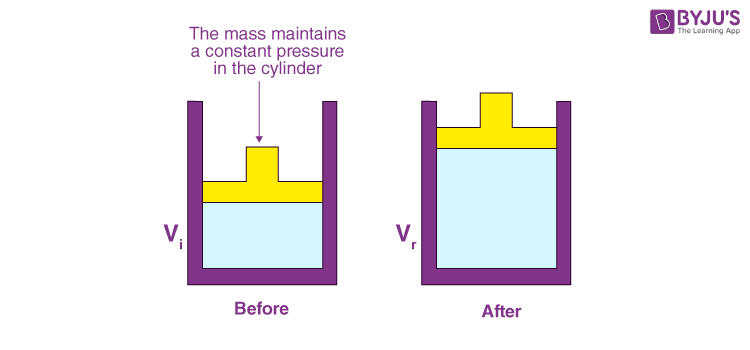
\includegraphics[width=0.75\textwidth]{isobaric.png}
    \caption{An example of an isobaric system. The gas pushes the mass and piston (surface area A) upward when heated.}
    \label{fig:isobaric}
\end{figure}

\subsection{Thermal Processes}
Systems will interact with their environment in several ways.
The \textit{thermal processes} described in this section are assumed to be \textbf{quasi-static}: changes occur slowly enough such that uniform pressure and temperature exist throughout all regions of the system at all times.

\subsubsection{Isobaric Processes}
\textbf{Isobaric processes are processes that occur at constant pressure}.
Consider the piston in Figure \ref{fig:isobaric}. 
Heating the gas causes it to expand from $V_i$ to $V_f$, doing work $W$ by lifting the piston and mass through displacement $\vec{s}$.
Because $W = Fs = (PA)s$, for all isobaric processes:

\[W = P\Delta V = P(V_f - V_i)\]

\subsubsection{Isochoric Processes}
\textbf{Isochoric processes are processes that occur at constant volume.}
While the pressure may increase and exert pressure on the walls of a container, by definition, $\Delta V = 0$, and therefore no work is done (via the above equation).
From the first law of thermodynamics, $\Delta U = Q$ for all isochoric processes.

\subsubsection{Isothermal Processes}
\textbf{Isothermal processes are processes that occur at constant temperature}.
For ideal gases, assuming constant number of moles, $P = \frac{nRT}{V}$.
Because pressure is now a function of volume, work can be solved for using the general form of work discussed below:

\[W = \int_{V_i}^{V_f} \frac{nRT}{V} = nRT (\ln{V}\Big|_{V_i}^{V_f}) = nRT\ln(\frac{V_f}{V_i})\]

Where does the energy for this work originate?
Since the internal energy of any ideal gas is proportional to its temperature ($U = \frac{3}{2}nRT$ for monatomic ideal gases), internal energy remains constant throughout the process.
Using the first law of thermodynamics, $\Delta U = Q - W \rightarrow Q = W$: the heat from the surroundings is used for work, or vice versa.

\subsubsection{Adiabatic Processes}
\textbf{Adibatic processes are processes where no heat is transfered between the surroundings and the system.}
Because $Q = 0$, $\Delta U = -W$.

For monatomic ideal gases, $\Delta U = \frac{3}{2}nR \Delta T$ as well, so $W = -\frac{3}{2}nR \Delta T$.

When an ideal gas expands adibatically, it does positive work, so W is positive.
Therefore, $T_i - T_f$ is positive, so the temperature of the gas decreases.
Similarly, if a ideal gas compresses adibatically, it does negative work, so the temperature of the gas increases.

It can be shown that $P_i V_i^\gamma = P_f V_f^\gamma$, where $\gamma = \frac{C_p}{C_v}$: the ratio specific heat capacities of the gas at constant pressure and constant volume.
(See 3.2.1 for a proof of this.)

\subsubsection{Other Processes}
Processes may be complicated enough that they may not be easily identifiable as one of the four processes just discussed.
However, correlary to the equation for isobaric processes, the following can be proven, assuming pressure is a function of volume:

\[W = \int_{V_i}^{V_f} P(V)dV\]

\subsection{Specific Heat Capacty of Gases}
Similar to how $Q = mc \Delta T$ for substances, a similar analog exists for gases:

\[Q = Cn\Delta T\]

$C$ (vs. $c$) refers to the \textbf{molar specific heat cpacity} (units $\frac{\textrm{J}}{\textrm{mol} \times \textrm{K}}$), and n analgously refers to the number of moles in the gas.
For gases, it is neccesary to differentiate between the molar specific heat capacaties for constant volume ($C_v$) and constant pressure ($C_p$).

To determine these heat capacities, we must first calculate Q needed to raise $T_i$ to $T_f$. According to the first law, $Q = \Delta U + W$.
For ideal gases, $\Delta U = \frac{3}{2}nR\Delta T$.
For constant pressure, $W = P\Delta V$.
According to the ideal gas law (holding pressure constant), $P\Delta V = nR \Delta T$, so $W = nR \Delta T$.
For constant volume, $W = 0$. So:

\[Q = \Delta U + W\]
\[Q_{\textrm{const. p}} = \frac{3}{2}nR\Delta T + nr \Delta T = \frac{5}{2}nR\Delta T\]
\[Q_{\textrm{const. v}} = \frac{3}{2}nR\Delta T + 0 = \frac{3}{2}nR\Delta T\]

Because $Q = Cn\Delta T$, $C = \frac{Q}{n\Delta T}$:
\[C_p = \frac{Q_{\textrm{const. p}}}{n\Delta T} = \frac{5}{2}R\]
\[C_v = \frac{Q_{\textrm{const. v}}}{n\Delta T} = \frac{3}{2}R\]

Thus, the ratio $\gamma$ between them (for monatomic ideal gases):
\[\gamma = \frac{C_p}{C_v} = \frac{\frac{5}{2}R}{\frac{3}{2}R} = \frac{5}{3}\]
Real monatomic gasses at STP show ratios similar to the theorized $\gamma = \frac{5}{3}$.

For diatomic ideal gases, molecules can exibit translational, rotational, and vibrational motion (vibrational at sufficently high temperatures).
For these gasses, it can be shown that $C_p = \frac{7}{2}R$, $C_v = \frac{5}{2}R$, and subsequently, $\gamma = \frac{7}{5}$.

It can be shown that for \textbf{all gases}:
\[C_p - C_v = R\]

\subsubsection{Proof of PV Relation for Adiabatic Processes*}
Assume that the gas changes by volume $\Delta V$ causing subsequent temperature change $\Delta T$.
From this, $\Delta W = P\Delta V$, and by the process being adiabatic, $\Delta Q = 0$.

\[\Delta U = C_v n \Delta T\]

From the first law:

\[\Delta U = C_v n \Delta T = Q - W = 0 - P\Delta V \rightarrow \Delta T = -\frac{P \Delta V}{C_v n}\]

From the ideal gas law (differiential)

\[\Delta (PV) = \Delta (nRT) \rightarrow P\Delta V + V \Delta P = nR \Delta T\]

Rearanging for $\Delta T$:

\[\Delta T = \frac{P\Delta V + V \Delta P}{Rn}\]

Setting both equations for $\Delta T$ equal:
\[\frac{P\Delta V + V \Delta P}{Rn} = -\frac{P \Delta V}{C_v n} \rightarrow C_v (P\Delta V + V\Delta P) + RP \Delta V = 0\]

Dividing by $PV$:
\[C_v (\frac{\Delta V}{V} + \frac{\Delta P}{P}) + \frac{R\Delta V}{V} = 0\]

Using $C_v = C_p - R$
\[C_v \frac{\Delta P}{P} + (C_p - R)\frac{\Delta V}{V} + \frac{R\Delta V}{V} = C_v \frac{\Delta P}{P} + C_p \frac{\Delta V}{V} = 0\]

\[C_v \frac{\Delta P}{P} + C_p \frac{\Delta V}{V} = \frac{\Delta P}{P} + \gamma \frac{\Delta V}{V} = 0 \textrm{ } (\gamma = \frac{C_p}{C_v})\] % yes i use a textrm for a space, cry about it

Thus, by intergration by parts:
\[\ln(P) + \gamma \ln(V) = \textrm{const}\]
\[PV^{\gamma} = \textrm{const}\]

Because this is true for all such processes, then we get the original relation:

\[P_i V_i^\gamma = P_f V_f^\gamma\]

\section{The Second Law of Thermodynamics}
\begin{definition}[The Second Law of Thermodynamics: Heat Flow]
    Heat flows spontaneously from a substance at higher temperature to a substance at lower temperature.
    Heat never flows spontaneously from a substance at lower temperature to a substance at a higher temperature.
\end{definition}

While the first law discusses the nature of heat and work relating to energy conservation, the second law is a statement about the natural tendency of hot to go to cold.

\subsection{Heat Engines}

One notable application of the second law are \textbf{heat engines.}
\begin{definition}[Heat Engines]
    A device that uses heat to perform work.
    Heat engines have three essential features:
    \begin{enumerate}
        \item \textit{Hot Reservoir}: a substance at a relatively high input temperature that supplies heat to the \textit{engine}.
        \item \textit{Engine}: an object that uses part of the input heat (through the \textit{working substance}) to perform work. (eg. the gasoline-air mixture in an automobile engine)
        \item \textit{Cold Reservoir}: where the remainder heat (not used by the engine) is rejected. Needs to have a lower temperature than the hot reservoir due to the second law.
    \end{enumerate}
\end{definition}

Efficent engines will produce a large amount of work from a small amount of input heat.
For 100\% efficent engines, all input heat will be converted to work.
That is, for input heat $|Q_h|$ and work $|W|$, \textbf{efficency} $e$ can be defined as the following:

\[e = \frac{|W|}{|Q_h|}\]

Like any other device, an engine still needs to follow the conservation of energy.
That is, for rejected heat $|Q_c|$:

\[|Q_h| = |W| + |Q_c|\]

Thus, efficency can also be written as

\[e = 1 - \frac{|Q_c|}{|Q_h|}\]

\subsubsection{Carnot's Principle}
\begin{definition}[Carnot's Principle, altnerate form of the Second Law of Thermodynamics]
    No irreversible engine operating between two reservoirs at constant temperatures can have greater efficiency than a \textbf{reversible engine} operating with the same temperatures.
    All reversible engines operating between the same two temperatures have the same efficiency.
\end{definition}


Reversible engines are engines whose processes are \textbf{reversible}: both the system and its environment can be returned to its original state.
In practice, no engines will function at this maximum efficency due to irreversible processes such as friction or heat transfer.
(Think about the second law; heat will go from hot to cold without any input, but will not go from cold to hot without input.)

Carnot's principle implies that the maximum efficency of a system is a function \textit{purely of the input and output temperatures}.
(Carnot's principle specifies \textit{two reservoirs at constant temperatures}.)
That is, the maximum efficency of an engine is: (It can be shown that $T_h$ and $T_c$ MUST be expressed in Kelvin.)

\[e_{max} = 1 - \frac{|Q_c|}{|Q_h|} = 1 - \frac{T_c}{T_h}\]

\textbf{Carnot's Principle does NOT state that reversible engines have 100\% efficency}.
If a process is reversible, then it will operate at the maximum efficency no matter what; even if that efficency is not 100\%.
(As no substance can reach a temperature of absolute zero, $\frac{T_c}{T_h}$ will always be greater than zero, and as such a perfectly 100\% engine cannot exist.)

\subsubsection{Refridgeration Processes}
By the second law, heat will always naturally flow from hot to cold.
Heat engines use this process to do work.
However, \textit{inverse heat engines work as well}: by providing work, heat can be made to flow from a cold reservoir to a hot reservoir.
Energy is still conserved throughout this process: $|Q_h| = |W| + |Q_c|$.
For ideal inverse heat engines (\textit{Carnot refridgerators}), the relation of max efficency still applies, in the same way.

Refrdigerators may be ranked how well they remove heat: that is, the coefficent of performance for refridgerators $= \frac{|Q_c|}{|W|}$.
Similarly, \textit{heat pumps} (devices that uses work to make heat out of cold outside air) may be ranked on how well they generate heat: the coefficent of performance for heat pumps $= \frac{|Q_h|}{|W|}$.

\subsection{Entropy}
When placing a hot object next to a cold object, heat is transfered to the cold object until both objects are in thermal equilibrium.
Compare this to using the hot and cold objects to run a heat engine, where work is also done.
As no work can be done using reservoirs in thermal equilibrium ($e = 1 - \frac{T_C}{T_H} = 0$), this flow of heat causes some \textit{permanent loss of ability to do work}.
Generally, all irreversible processes cause at least some permanent loss.

More formally, consider the "equation of max efficency", $\frac{Q_C}{Q_H} = \frac{T_C}{T_H}$.
This can be rearranged to form $\frac{Q_C}{T_C} = \frac{Q_H}{T_H}$.
The quantity $\frac{Q}{T}$ is \textbf{the change in entropy} $\Delta S$ (SI unit $\frac{J}{K}$, kelvin SPECIFICALLY) for any reversible process at a constant temperature.
Like internal energy, entropy is a function of state.
Entropy is negative when heat leaves the object, and positive when heat enters the object.
The difference between the loss and gain of entropy is the permanent loss of ability to do work.
\textit{Reversible processes do not cause any entropy loss:} $\Delta S_{universe} = 0$.

\[\Delta S_C + \Delta S_H = +\frac{Q_C}{T_C} - \frac{Q_H}{T_H} = 0\]



\section{The Third Law of Thermodynamics}
\begin{definition}[The Third Law of Thermodynamics]
    It is not possible to lower the temperature of any system to absolute zero ($T = 0\textrm{K}$) or below in a finite number of steps.
\end{definition}



\end{document}